\documentclass[sigchi-a, authorversion]{acmart}
\usepackage{booktabs} % For formal tables
\usepackage{ccicons}  % For Creative Commons citation icons

% Copyright
\setcopyright{none}
%\setcopyright{acmcopyright}
%\setcopyright{acmlicensed}
%\setcopyright{rightsretained}
%\setcopyright{usgov}
%\setcopyright{usgovmixed}
%\setcopyright{cagov}
%\setcopyright{cagovmixed}
\renewcommand\footnotetextcopyrightpermission[1]{} % Removes ACM copyright line (non-archival Workshops)

\settopmatter{printccs = false, printacmref = false}
% DOI
\acmDOI{10.475/123_4}

% ISBN
\acmISBN{123-4567-24-567/08/06}

%Conference
\acmConference[Sensemaking Workshop: CHI 2018]{CHI 2018}{April 2018}{Montr\'eal, Canada}
\acmYear{2018}
% \copyrightyear{2018}

\acmPrice{15.00}

%\acmBadgeL[http://ctuning.org/ae/ppopp2016.html]{ae-logo}
%\acmBadgeR[http://ctuning.org/ae/ppopp2016.html]{ae-logo}

\begin{document}
\title{The Need for Sensemaking in Networked Privacy and Algorithmic Responsibility}

\author{Max Van Kleek}
\affiliation{%
  \institution{University of Oxford}
  \city{Oxford}
  \postcode{OX1 3QD}
  \country{United Kingdom} }
\email{max.van.kleek@cs.ox.ac.uk}

\author{William Seymour}
\affiliation{%
  \institution{University of Oxford}
  \city{Oxford}
  \postcode{OX1 3QD}
  \country{United Kingdom} }
\email{william.seymour@cs.ox.ac.uk}

\author{Michael Veale}
\orcid{0000-0002-2342-8785}
\affiliation{%
  \institution{University College London}
  \city{London}
  \postcode{WC1E 6BT}
  \country{United Kingdom}}
\email{m.veale@ucl.ac.uk}

\author{Reuben Binns}
\affiliation{%
  \institution{University of Oxford}
  \city{Oxford}
  \postcode{OX1 3QD}
  \country{United Kingdom} }
\email{reuben.binns@cs.ox.ac.uk}

\author{Nigel Shadbolt}
\affiliation{%
  \institution{University of Oxford}
  \city{Oxford}
  \postcode{OX1 3QD}
  \country{United Kingdom} }
\email{nigel.shadbolt@cs.ox.ac.uk}


% The default list of authors is too long for headers.
\renewcommand{\shortauthors}{M. Van Kleek et al.}


%
% The code below should be generated by the tool at
% http://dl.acm.org/ccs.cfm
% Please copy and paste the code instead of the example below.
%
% \begin{CCSXML}
% <ccs2012>
%  <concept>
%   <concept_id>10010520.10010553.10010562</concept_id>
%   <concept_desc>Computer systems organization~Embedded systems</concept_desc>
%   <concept_significance>500</concept_significance>
%  </concept>
%  <concept>
%   <concept_id>10010520.10010575.10010755</concept_id>
%   <concept_desc>Computer systems organization~Redundancy</concept_desc>
%   <concept_significance>300</concept_significance>
%  </concept>
%  <concept>
%   <concept_id>10010520.10010553.10010554</concept_id>
%   <concept_desc>Computer systems organization~Robotics</concept_desc>
%   <concept_significance>100</concept_significance>
%  </concept>
%  <concept>
%   <concept_id>10003033.10003083.10003095</concept_id>
%   <concept_desc>Networks~Network reliability</concept_desc>
%   <concept_significance>100</concept_significance>
%  </concept>
% </ccs2012>
% \end{CCSXML}

% \ccsdesc[500]{Computer systems organization~Embedded systems}
% \ccsdesc[300]{Computer systems organization~Redundancy}
% \ccsdesc{Computer systems organization~Robotics}
% \ccsdesc[100]{Networks~Network reliability}

\begin{CCSXML}
<ccs2012>
<concept>
<concept_id>10003120.10003123.10011758</concept_id>
<concept_desc>Human-centered computing~Interaction design theory, concepts and paradigms</concept_desc>
<concept_significance>500</concept_significance>
</concept>
</ccs2012>
\end{CCSXML}

\ccsdesc[500]{Human-centered computing~Interaction design theory, concepts and paradigms}

\begin{abstract}
	This paper proposes that two significant and emerging problems facing 
    our connected, data-driven society may be more effectively solved by being
    framed as sensemaking challenges. The first is in empowering individuals 
    to take control of their privacy, in device-rich information environments
    where personal information is fed transparently to complex networks of information brokers.  
    Although sensemaking is often framed as an analytical activity undertaken by experts, due to the fact that 
    non-specialist end-users are now being forced to make expert-like decisions 
    in complex information environments, we argue that it is both appropriate and
    important to consider sensemaking challenges in this context. The second is 
    in supporting human-in-the-loop algorithmic decision-making, in which important decisions bringing 
    direct consequences for individuals, or indirect consequences for groups, are made with the 
    support of data-driven algorithmic systems.  In both privacy and algorithmic decision-making, 
    framing the problems as sensemaking challenges acknowledges complex and ill-defined problem 
    structures, and affords the opportunity to view these activities as both building up
    relevant expertise schemas over time, and being driven potentially by recognition-primed 
    decision making.
    
    % In such varied domains as recidivism, predictive policing, algorithmic insurance, loans, and	pricing, people play vital roles in both administering and taking responsibility for the    recommendations made by these algorithms.  
    
    % In many cases, it is critical to ensure that such decisions are made fairly, despite the potential for underlying biases in the data  or algorithms within them.
%   UPDATED---\today. This sample paper describes the formatting
%   requirements for SIGCHI Extended Abstract Format, and this sample
%   file offers recommendations on writing for the worldwide SIGCHI
%   readership. Please review this document even if you have submitted
%   to SIGCHI conferences before, as some format details have changed
%   relative to previous years. Abstracts should be about 150
%   words. Required.
\end{abstract}

\keywords{Sensemaking; end-user privacy; transparency; fair and accountable machine learning.}

\maketitle
% \begin{sidebar}
%   \textbf{Good Utilization of the Side Bar}

%   \textbf{Preparation:} Do not change the margin
%   dimensions and do not flow the margin text to the
%   next page.

%   \textbf{Materials:} The margin box must not intrude
%   or overflow into the header or the footer, or the gutter space
%   between the margin paragraph and the main left column.

%   \textbf{Images \& Figures:} Practically anything
%   can be put in the margin if it fits. Use the
%   \texttt{{\textbackslash}marginparwidth} constant to set the
%   width of the figure, table, minipage, or whatever you are trying
%   to fit in this skinny space.

%   \caption{This is the optional caption}
%   \label{bar:sidebar}
% \end{sidebar}

% \begin{figure}
%   
\includegraphics[width=\marginparwidth]{sigchi-logo}
%   \caption{Insert a caption below each figure.}
%   \label{fig:sample}
% \end{figure}


\section{Introduction}
As society has become data-centric, routinely and effectively making sense of it all is increasingly important. Decisions seemingly grounded in new forms of data are pervasive, embedded and on occasion critical. The role of case-specific, digitised evidence has become heightened in high-stakes contexts where outcomes may affect a decision-subject and/or the decision-maker herself. Non-specialists are increasingly forced to perform as expert data analysts in their roles as teachers, doctors, police supervisors, courtroom judges, or retail store managers---all without traditional training.  Even outside employment contexts, people often need to make complex, multi-criteria decisions with many factors and an abundance of choice. Increasing trends towards self-tracking through wearable, portable, and embedded smart devices compound this.

\emph{Sensemaking} unsurprisingly focuses on studying the set of activities pertaining to \emph{making sense} of information, including identifying relationships, properties, or patterns~\cite{pirolli2005sensemaking}.  Research in sensemaking within HCI has focused both on characterising how people (usually experts) perform sensemaking in various domains or contexts of interest, as well as on supporting the activities of sensemaking through interaction techniques and methods embodied in tools for visualising, exploring and interrogating complex information spaces.  In this position paper, we propose that the study of sensemaking is now not only more important than ever, but relevant to new contexts outside those of traditional intelligence and data analyst roles. We focus on two: citizens making routine decisions about their privacy in networked environments, and those using predictive algorithmic systems to make consequential decisions about others.

% become correspondingly more important. Two domains that this paper argues
% are of particular urgency relate to privacy, and the pervasive (both public and private-sector)
% se of machine learning and data-driven algorithms in supporting decisions affecting individuals.
% We describe each of these separately below.

\section{Networked Privacy and Sensemaking}

In our research, we focus on networked privacy: understanding ways to support people's privacy preferences in a world full of devices that capture, use, and transmit personal data for various purposes.
While the market of two of these kinds of devices---smartphones and wearables---is already enormous, it nonetheless continues to grow.  Meanwhile, ``Internet of Things'' (IoT) devices, including ``smart'' connected home devices are seen by market analysts as being on the brink of becoming ubiquitous in people's homes.  Smart speakers with voice assistants such as Amazon's Echo or Google Home in particular can already be found in nearly 20\% of US households~\cite{smartspeaker}. 

In networked social environments, privacy is already a dynamic and contextual process, where individuals who are aware that information can be disseminated fast, rely on their heuristic understanding of the network and social norms and ties to manage information flows~\cite{marwick2014networked}. In the more automated and hidden data transmission common to many kinds of data-capturing devices, the privacy problem is challenging for several further reasons.  Moreover, data from these devices is often generic enough in form to allow heavy re-purposing later.  The data may be shared with many kind s of first- and third- party data brokers in the process of being processed or used.  Each such data broker may itself may have different privacy policies, security practices, and may be subject to different (or no) data protection laws in different jurisdictions within which they fall, with different levels of practical enforcement.  

Compounding the problem of empowering end-users in privacy decision-making is often a lack of knowledge--even about what data about them is being captured and how it is being used.  This lack of \emph{a priori} understanding means that they also have little basis upon which to understand or interpret these activities. In the language of sensemaking, end-users currently lack necessary schemas and scaffolding for them to act as experts, so as to effectively recognise patterns in data collection activities that violate their specific privacy expectations or preferences.  The lack of an understanding also leads people to be unable to effectively articulate preferences in ways that can be translated into effective interventions. One example of an area where expertise can help is in understanding the relationship between kinds of data collection and the potential privacy implications such activities may pose. For instance, while something as simple as disclosure of a device identifier may seem innocuous, it may later be realised that such an identifier is the method by which users' activities are collated multiple apps and devices, and used for targeted advertising or re-identification.

Our preliminary results, which we describe in further detail below, suggest that such preferences are only formed incrementally as people learn more about typical data handling practices and their implications.  As people form such preferences, they tend to be idiosyncratic. Far from being one-size-fits-all, or generalisable to groups, many people will be against or for about particular uses for their data, or for or against particular companies applying such uses in particular ways. Such preferences seem to be grounded in norms, popular perceptions, and past experiences, suggesting the need for people themselves to become experts of their own privacy preferences before such preferences can be operationalised.

% \subsection{Privacy as Sensemaking}
% Privacy is notoriously difficult to define
% Attempts to quantify privacy have been frought with difficulties.
% \subsection{Privacy as Sensemaking}

\subsection{The \emph{X-Ray Project}}

We anticipated that empowering people to take control of their privacy would require a 
multi-stage sensemaking process. The first, \emph{evidence gathering}, would for privacy
consist of viewing and examining the ``ground truth'', that is, the data collection 
activities occurring within their information ecosystems.  The second stage, corresponding
to \emph{schema formation}, we envisioned would be when expectations and preferences would
start to be formed, based on understanding the data collection practices.  These expectations
would also have to include connecting activities to potential risks and privacy implications. 
In the third stage, such preferences and needs would be exercised, first, by being able to 
anticipate risks and exposure consequences of actions before they occur, and two, being 
able to map goals to strategies for regaining privacy (e.g. the use of particular apps, devices or privacy settings).

To support this sensemaking process, we designed an interface framework called \emph{X-Ray Refine}, 
which we describe next.  
% \emph{X-Ray Refine}  data collection activities of the
% apps and devices they used, and the ways that these translate to individuals' overall
% information exposure to first- and third- parties. 

\subsubsection{X-Ray Refine}

\begin{figure*}[b]
  \centering
  \setlength\fboxsep{0pt}
  \setlength\fboxrule{0pt}
  \fbox{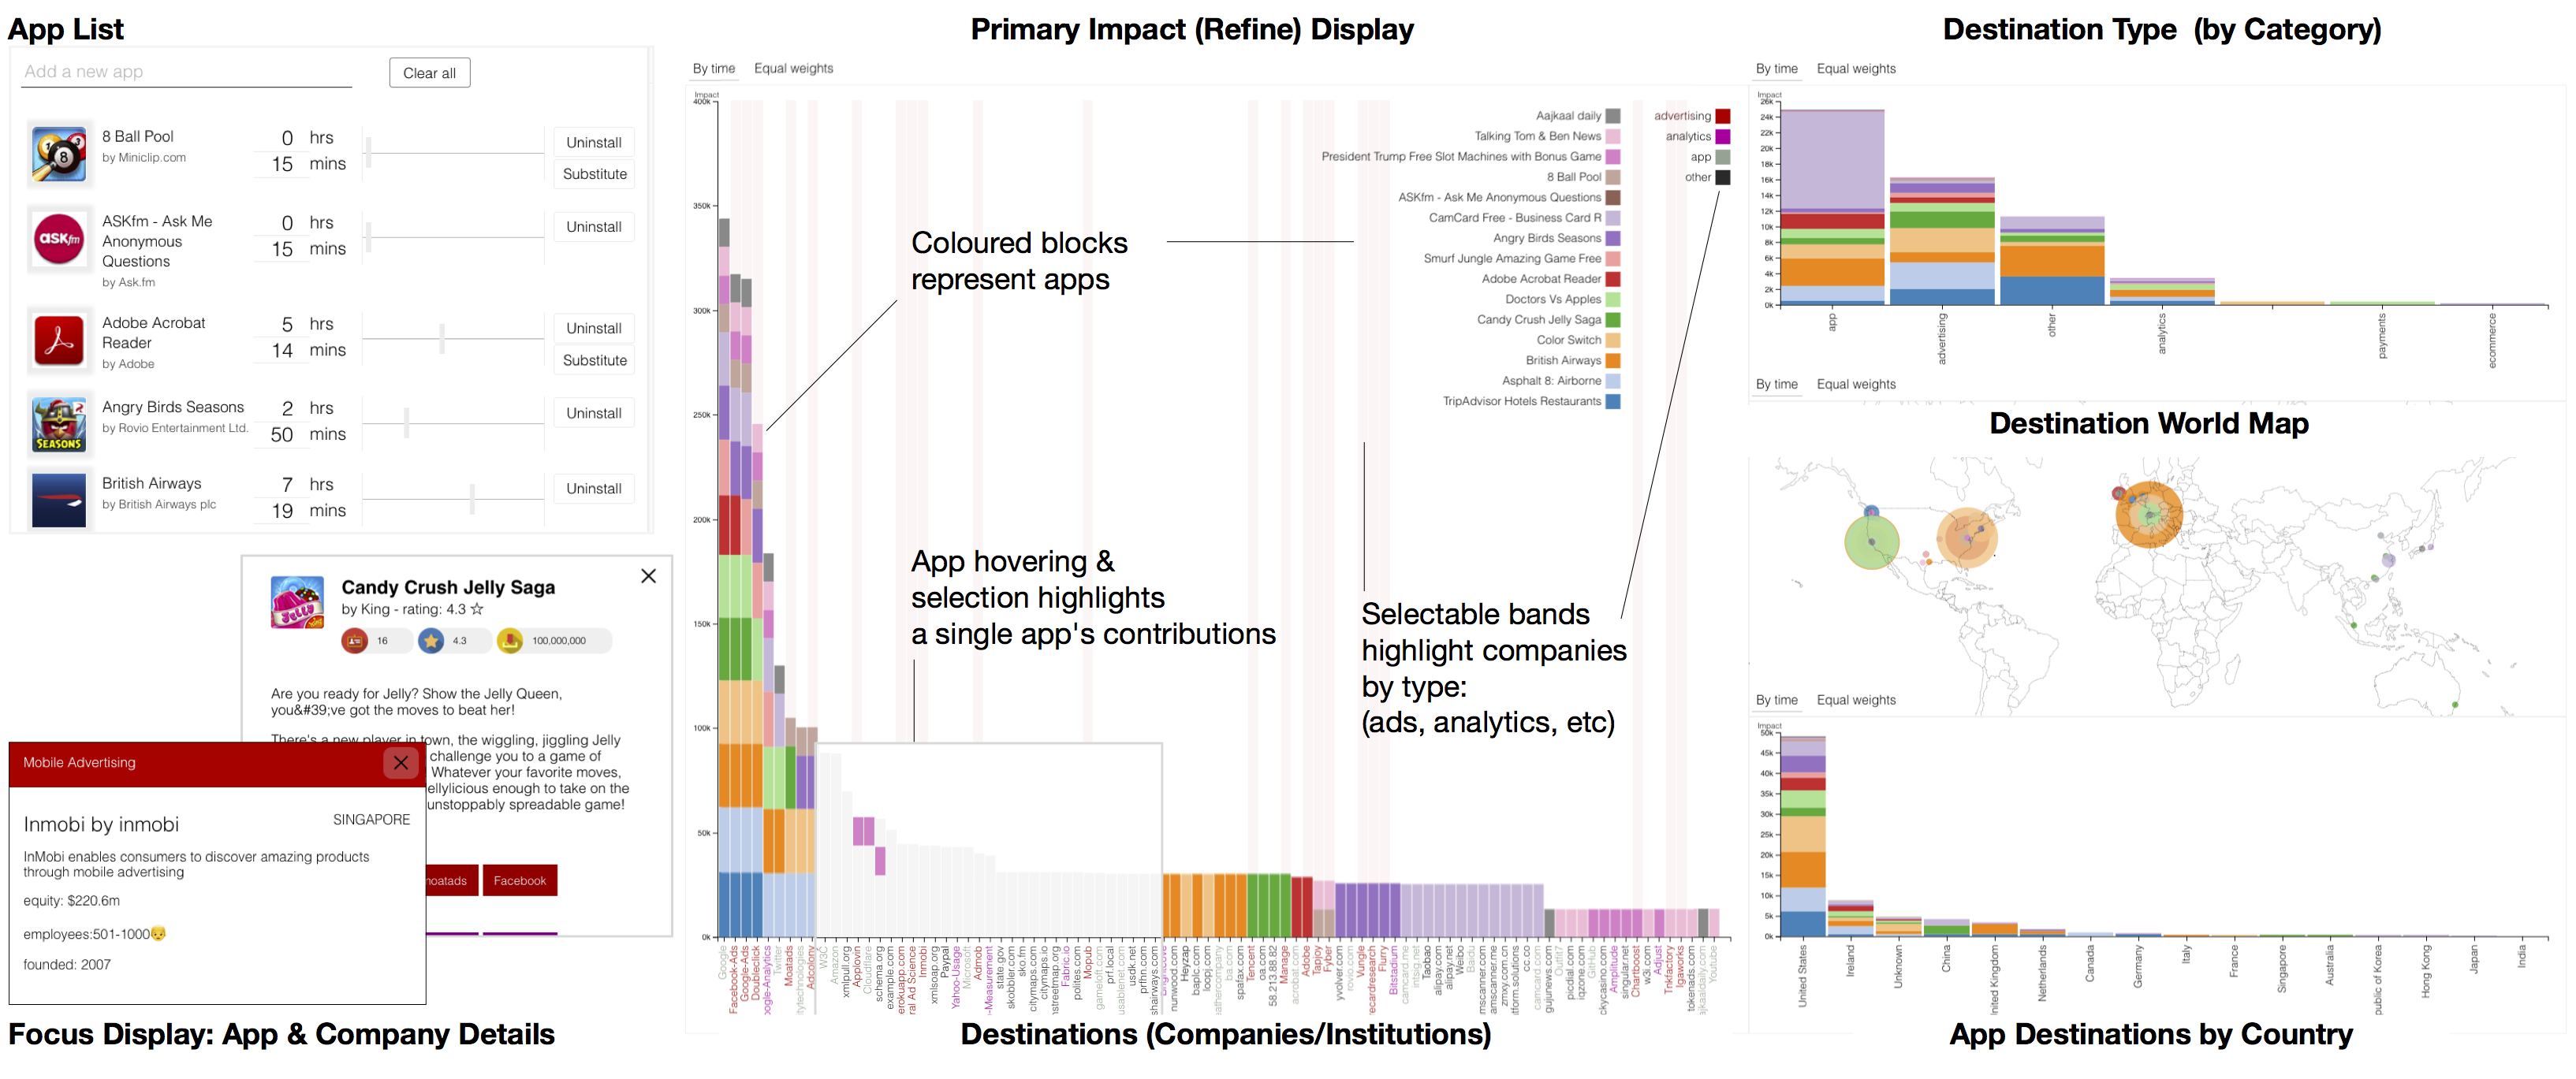
\includegraphics[width=7.2in]{super_main1}}
  % \fbox{\includegraphics[width=7.5in]{refine_procedure}}

  \caption{\emph{X-Ray Refine}. The \emph{exposure profile} view consists
  of a stacked bar chart showing the impact contribution of each app,
  with destinations along the x-axis (sorted from most to least). 
  Hovering over an app (in the legend) highlights the contribution of that app to the profile. Clicking
  on an app produces a focus display containing app details; clicking on a 
  company name invokes a focus that displays destination details, if known. 
  Hovering over app types highlight destinations of that type (e.g. advertisement, analytics, app
  functionality, etc). Supporting views show contributions by type, and 
  location.}

  \label{f7}
\end{figure*}

X-Ray Refine is our prototype interface for supporting sensemaking of 
information collection by connected devices and apps,  It consists of 
an information exposure profile, derived through an analysis of 
the information sensing, processing and dissemination activities~\cite{btdchi} of 
both software and hardware in their information ecosystem.   
In its current instantiation, \emph{X-Ray Refine} has models for over 2 million 
Android apps derived through static bytecode analysis~\cite{refine};  work is currently 
underway to support more apps, iOS, and smart home devices.

The main interface comprises a multi-view focus-plus context display
that supports exploring a model of a person's complete information exposure
using multiple views and perspectives. One of the main views is an exposure 
profile chart, which consists of a stacked bar that visualises the 
amount of information being transmitted by each app or device to each
respective data controller.  From this overview, the user can pivot or
explore in depth along the following dimensions:

\begin{enumerate}
\item \emph{Apps/devices}: each app's contributions to a particular aspect of exposure.
\item \emph{Data uses}: the purpose(s) the data are being collected by each controller
\item \emph{Data type}: the kinds of data that are being sent to each controller by each source\footnote{This functionality is currently only available for a limited number of apps due to limitations of our analytical methods}
\item \emph{Data controllers}: Details of each company/organisation collecting the information.
\item \emph{Geographic destinations}: The first-hop destinations (to city granularity) of where data are going
\item \emph{Data Jurisdiction}: The jurisdictions under which data collected and kept fall within.
\end{enumerate}

The interface is meant to allow individuals to explore their exposure starting
with any of the above dimensions to any others seamlessly without losing context.
To do this, focusing and filtering are coordinated across views, which may
be switched into the main view at any time.

\subsubsection{Study results}

A lab study of Refine (described in detail in a paper at CHI 2018~\cite{refine}) 
found substantial evidence that supported the view that participants engaged in
sensemaking activities whilst using Refine, and that they were able to effectively 
achieve a baseline understanding of their information exposure.  For most participants,
such an understanding was altogether new, or at least contained many aspects that were
seen as unexpected and surprising.  

For a majority of participants, we saw support for the second phase---participants were able
to identify patterns during their exploration that let them form a view of the complex
mesh of data collection activities being portrayed.  For example, most participants were able
to start to identify norms and exceptions among the apps they used, that is, apps that seemed
``typical'',  proportional or well-justified, versus those that they considered suspect.  

From this, a most participants were able to progress to the third stage, in which they were 
able to formulate and articulate specific privacy preferences, goals, and strategies to 
achieve them. Many expressed frustration at the lack of options they had to control or 
mitigate some of the data collection activities, which, in turn, limited their ability 
to devise strategies that would not involve forced tradeoffs--such as forfeiting the use of 
an app or device altogether. Despite common views and frustrations, however, many of the specific privacy goals and views varied considerably among individuals. For instance, while some viewed large platforms such as Google and Facebook as most trustworthy and worthy of their data, this was 
often due to many different reasons, from the sheer pervasiveness of these platforms, to expecting
such platforms to be subject to greater scrutiny.  Others, however, had other opinions, such as
viewed such platforms as a primary threat to their privacy.  Still others did not focus on platforms per se, but on the jurisdictions that they were based; one participant in particular who, herself, had left China at a young age, expressed the desire to never have her data go to any Chinese companies, or  companies that would place her data within the reach of the Chinese government.  Such specific and idiosyncratic privacy preferences we saw in the study support our view of the need to have end-users able to devise their own personal privacy goals, which we see as only achievable through understanding.

% * <m.veale@ucl.ac.uk> 2018-03-01T21:16:01.024Z:
% 
% > Note
% note what?
% 
% ^.

\section{Human-in-the-loop Algorithmic Decision-making}

%% a short background paragraph here about kinds of algorithmic decisions being made by  machines

The sheer amount of structured data available to many organisations when making decisions is often beyond easy human comprehension (or sensemaking?). Thus, most have turned to algorithms to `digest' data firehoses into aggregated analyses which can be used to inform decision makers. However, great care needs to be taken when the decisions being made have large personal effects on those they concern. A commonly used example of a scenario with obvious human impact in the literature is recidivism predictors, which produce risk scores for defendants that are then used to inform some decision, ranging from sentence plans and resource allocation within prisons~\cite{mooreOASys}, to bail~\cite{marionHART17} or parole~\cite{propublicamachinebias} decisions.

A major potential harm in these situations comes from the possibility that automated processes might result in unfair outcomes. While it is certainly true that humans are capable of making biased decisions on an institutional scale, the ease with which an algorithm can become biased through design or training warrants deeper scrutiny~\cite{binns2017like}. To this end, European data protection law, soon to be strengthened by the European General Data Protection Regulation (GDPR), includes a clause which gives data subjects the right not to be subject to decisions which produce significant effects and are performed entirely automatically (now Article 22)~\cite{edwardsveale}.

With this in mind, it becomes apparent that the task of a person who is making algorithm-assisted decisions (the ``human in the loop'') requires sophisticated sensemaking in order to interpret results from automated systems, and to make an evaluation as to whether the suggested outcomes are fair or otherwise should be challenged. In part, this might be related to understanding whether the system is performing within normal parameters, or acting as expected. But it might also relate to challenging the model structure as a whole, and noticing it is problematic in some value laden manner. The phenomena or data flows being modelled might be changing over time, and sensemaking might involve understanding such change as and when it happens. 

Finally, communicating and justifying the reasoning behind a decision arrived at by an algorithm is extremely tricky given wildly varying subjective thresholds concerning what constitutes appropriate grounds for a negative outcome~\cite{binns2018reducing}.

\subsection{Definitions of Fairness}

%this section shows the need for having the human in the loop

What does it mean for an algorithmic decision to be unfair? While we have largely unified societal intuitions about what is fair, translating this into something which can be understood by a machine proves to be far more difficult. Too often, the question as to whether it is even possible to conceptualise right and wrong using statistics is just assumed to be yes. Yet as fairness is often something that people ``know when they see it'' (and don't always agree upon), checking whether complex and subjective statistical systems demonstrate fairness robustly and throughout is tricky.

Reasoning about statistical fairness criteria often coalesces along lines of legally protected characteristics (such as race), as these are where the most glaring problems are often to be found~\cite{barocas2016big}. But just ticking boxes derived from existing legislation as a model variable specification tends not to work, as other characteristics can act as proxies or indicatiors for protected ones (for example, postcode is often correlated with race). This connects to the idea of indirect discrimination (EU) or disparate impact (US). Common fairness metrics include those on the more blunt end of the spectrum, such as ensuring parity amongst protected groups regardless of the differences between them. More sophisticated approaches proposed involve equalising accuracy or false positive/negative rates between groups, but the impact of these methods is limited as it entails an unsolvable three-way trade-off \cite{chouldechova2017fair}. Yet these metrics are distant and likely arcane to decision-subjects and decision-support users, and to make sense of the fairness of systems in order to work towards legitimacy or political debate seems challenging. Moreover, other researchers have considered representational harms---how individuals or concepts are represented in datasets, such as those used in natural language processing, which contain common and often undesirable stereotypes~\cite{BolukbasiCZSK16a}---and found these difficult to grapple with. Notions of `debiasing' have been criticised here, as the way humans understand fairness in language seems difficult to reduce to concepts such as computational geometry. 

Time and again we see that effectively operationalising fairness is something that lies beyond the current reach of machine learning. This situation is not helped by the fact that (from a logical perspective), human distinctions between fairness and unfairness are often contradictory. Indeed, as philosophical accounts attest, the concept of fairness is multifaceted and divisible into different dimensions~\cite{binns2017fairness}. Coupled with the fact that avoiding mistreatment often needs to be balanced with respect to several different types of protected groups (race \textit{and} gender \textit{and} age etc.), this means that even for a human, making fair decisions is a daunting and technically complex task, especially when the commonly held view of algorithmic decisions is one of objective neutrality. 

Unfairness in machine learning systems can arise from many sources---entrenched social structures, data sampling, categorisation---the role and responsibility of an algorithmic system in the wider societal responsibility for unfairness is unclear. Do systems need to be non-discriminatory? Should operators try to compensate for discrimination that exists in wider society? In what way and to what extent? To work this out is a political problem, and one which requires understanding of the context, datasets, and wider social dynamics. Not only that, but fairness is also not a one-shot challenge, but a complex and shifting notion that not only has to be managed over time, but where the legitimacy of the solution is perhaps as much driven (or undermined) by process as it is by outcome~\cite{Pasquale:2014vt}.

% can legal definitions help? no
% cite reuben/will fairness means lots of things
% cite michael's unfairness comes from lots of sources
% achieving fairness is a process not a one-shot deal

\subsection{Algorithmic Explanations as Sensemaking}

In order to grapple with value-laden decision-making, practitioners both individually and collectively need to build up mental models of the decision support systems that they work with. These schemas allow for more nuanced evidence than the raw yes/no output from the algorithm. In cases where algorithms are being used to make more open ended decisions, being able to spot situations where algorithmic output is expected to be flawed is of real value in shaping questions and further examination. An example of this might be a predictive policing system exaggerating the risk of crime in a area immediately following a festival or carnival. If operators understand (or infer) that the system makes use of incident rates from previous months, then they can interpret, or even predict, its output accordingly. This kind of sensemaking is already seen in practice~\cite{vealefairnessdesign2018}, but we have little knowledge on when and if it works given the variety of tasks required in high-stakes settings, and how it might be best fostered through design. Crucially, practitioners are much more likely to go against the decision of an algorithm if they have a reasonable argument as to why the algorithm is incorrect, rather than just an intuition that the decision reached is unfair. There is likely even a legal requirement for this, as systems that wish to avoid higher levels of regulation in Europe by showing they are not fully automated will need to show that the users have the ``authority and competence'' to challenge the system, as well as demonstrate that they do not ``routinely [apply]'' the results~\cite{vealeedwardsa29}.  If the hype towards trusting data-driven systems continues in the business sector at the same or greater rate than the growth in system efficacy, this problem will likely only get worse, as among non-technical users it is easy to delegate authority to an arcane, ``sophisticated'' and likely expensive system, even when it is unproven.

Building systems which are able to offer some insight into their reasoning can play a big part in speeding up the sensemaking process for practitioners. One can build a surprisingly effective mental schema based on an algorithm's decisions, and the reasons for making those decisions backed up by examples of similar cases. In particular, where the users are already domain experts, they are often not learning from scratch but from lived experience in this area, and may see parallels (or distinctions) not captured by the system. Cases can also provide the evidence needed by decision makers to overturn a system's decisions with confidence, and avoid automation bias and over-reliance~\cite{Skitka:1999il}. But extracting this type of reasoning from an algorithm is not an easy task. The methods which are most widely applicable operate as ``black boxes'', performing analysis on input and output without ever seeing inside the mechanisms that make decisions (such as \cite{ribeiro2016should}). This really emphasises the need for practitioners to develop sound mental models as a way of understanding what an algorithm is doing through the window offered by black box explanations. The cases that are put in front of a system are less likely to be uncommon, edge cases on which issues of fairness, model certainty and due process are likely to be stressed. 

Lastly, the relevance of any explanation systems to determinations of fairness is unclear. If we see fairness as a global property of the model, defined in terms of some comparison between different groups amongst a population of decision subjects, then an explanation of an individual decision may not help decision-makers to make fairness judgements. Insofar as sensemaking arises from individual, snapshot interactions with a system, the extent to which we can design for the assessment and monitoring of fairness resembles the ancient Indian tale of the blind men and the elephant: users of this system might each get a different, local glimpse into the workings of a model for which we hope fairness is a global property. They might even perceive their glimpse differently from each other. Given data-driven systems are often deployed within institutions (both formal organisations and informal, repeated human norms, rules and shared strategies~\cite{crawford1995grammar}), this adds a further level to sensemaking needs: is it possible for design to promote sensemaking at an aggregated organisational level, as well as an individual level? What would this entail?



%-> decision makers need to form mental models of the algorithms which are assisting them (expertise schema?)

% what would framing machine learning-based decisions as 
% looking like?  literal expertise schemas building up
% over time 

% important to give critique of the idea that local explanations can help understand fairness issues. info you get from local explanations is quite disconnected from fairness metrics

\section{Conclusion}

In this paper, we have presented preliminary work towards applying sensemaking to address two challenges we believe are significant for achieving a healthy and fair digital society. The first is in helping people to bring the data collection activities of their increasingly connected environments in line with their privacy preferences---a goal which we argue can only be achieved by allowing people to better form such preferences first.  Our study of a prototype sensemaking tool, X-Ray Refine, found that supporting end-users in gaining a baseline understanding of the data sharing and usage activities, risks, opportunities and norms of their information environments did ultimately help them better articulate their privacy goals, and strategies to achieve them.  The resulting preferences can be highly varied, suggesting that it is important for individuals to engage in such activities themselves. 

The second is in both using, and being subject to, decisions made and supported by machine learning-based algorithmic systems. The need to make sense of these complex systems is fast moving from expert to lay domains, at the same time as the quality of the complexities involved is changing and, in some ways, becoming more daunting. Framing the challenge as one of sensemaking provides the opportunity to consider not only the means by which users (and subjects) of these systems may be supported in understanding them, but also the empirical and theoretical adaptations required to deal with these changes. Such adaptations will invariably play an important role in informing not only designers, but regulators, policy-makers, civil society and individual users as such systems become pervasive throughout society.

% In this paper, we have presented preliminary work towards applying the idea and theory of sensemaking to two areas we believe are important towards improving individuals' ability to interact with data. These are in managing personal privacy preferences and their deployment in a complex, networked world, and in both using and being subject to decisions made and supported by machine learning--based algorithmic systems. The need to make sense of complex systems is fast moving from expert to lay domains, at the same time as the quality of the complexities involved is changing and, in some ways, becoming more daunting. The field of sensemaking must consider the empirical and theoretical adaptations required to deal with these changes, which will play an important role in informing not only designers, but regulators, policy-makers, civil society and individual users.


\bibliography{sample-bibliography}
\bibliographystyle{ACM-Reference-Format}

\end{document}
